\lecture{13}{Преобразование Фурье. FFT.}
\subsection{Дискретное преобразование Фурье.}
Пусть у нас есть некоторый набор коэффициентов (значений) $x_{i}, i = 0\ldots N - 1$

По своей сути, дискретное преобразование Фурье --- преобразование одного набора коэффициентов (значений) 
в другой набор по формуле:
\[
  X_{k} = \sum_{n=0}^{N - 1} x_{n} e^{\frac{-2\pi i}{N} kn}
.\] 

Давайте разберёмся, в чём смысл этой формулы (следующую часть с картинками можно пропустить, если вы
торопитесь и не хотите особо вникать, все картинки взяты с \href{https://www.youtube.com/watch?v=spUNpyF58BY}{замечательного видео}).

Сделаем оговорку, что дискретное преобразование Фурье обычно применяют к функциям от некоторого параметра
$t$ (можно воспринимать его как время, например, при анализе сигналов), эти функции мы и дискретизируем с
некоторой точностью и получаем исходный набор значений. К нему и применяется преобразование.

Для начала рассмотрим комплексную плоскость и вектор $e^{ik}$:
 \begin{figure}[H]    
  \centering    
  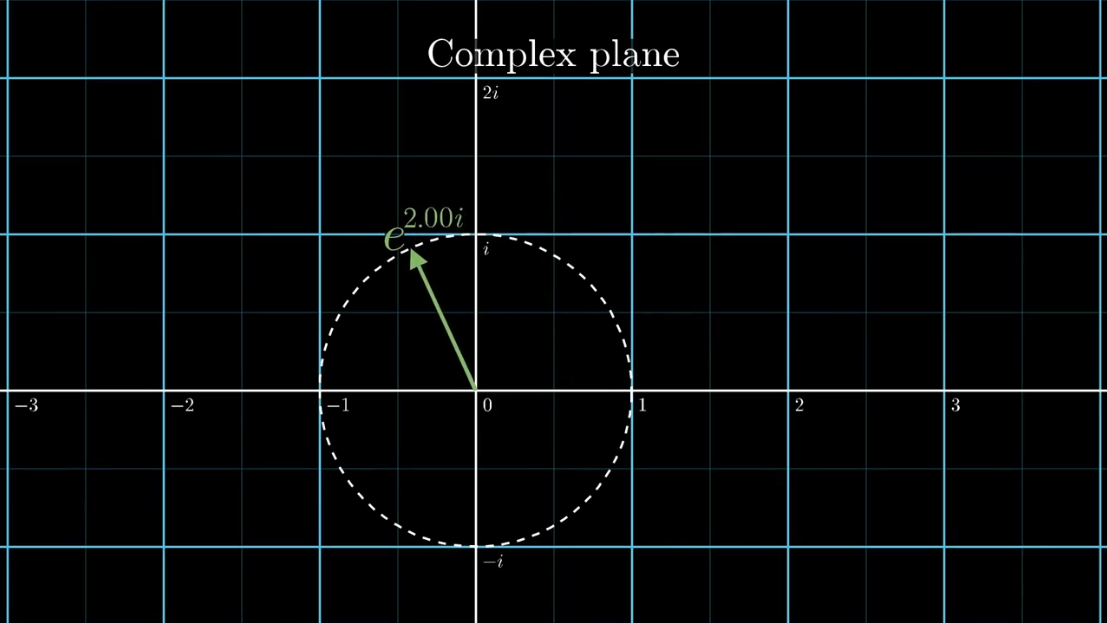
\includegraphics[width=0.8\textwidth]{figures/dft1.png}    
  \caption*{Вектор $e^{ik}$ на комплексной плоскости.}        
\end{figure} 

Как известно из формулы Эйлера, этот вектор будет описывать окружность при повороте (изменении $k$).
Далее перепишем для удобства $k = 2\pi t$, где $t$ можно воспринимать как время (про применение дискретного
преобразования поговорим позже, там оно понадобится).

\begin{figure}[H]    
  \centering    
  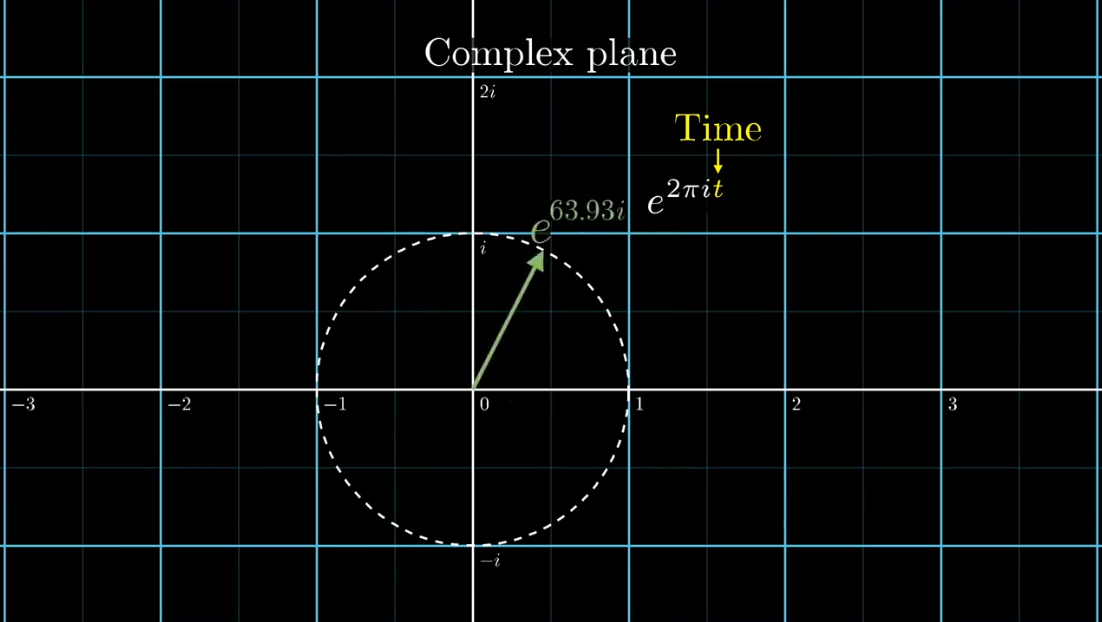
\includegraphics[width=0.8\textwidth]{figures/dft2.png}    
  \caption*{Сделаем замену $k = 2\pi t$.}        
\end{figure} 

Теперь добавим множитель $f$ в степень, чтобы регулировать <<скорость поворота>> вектора. Также добавим
знак $-$ в степень по соглашению.

 \begin{figure}[H]    
  \centering    
  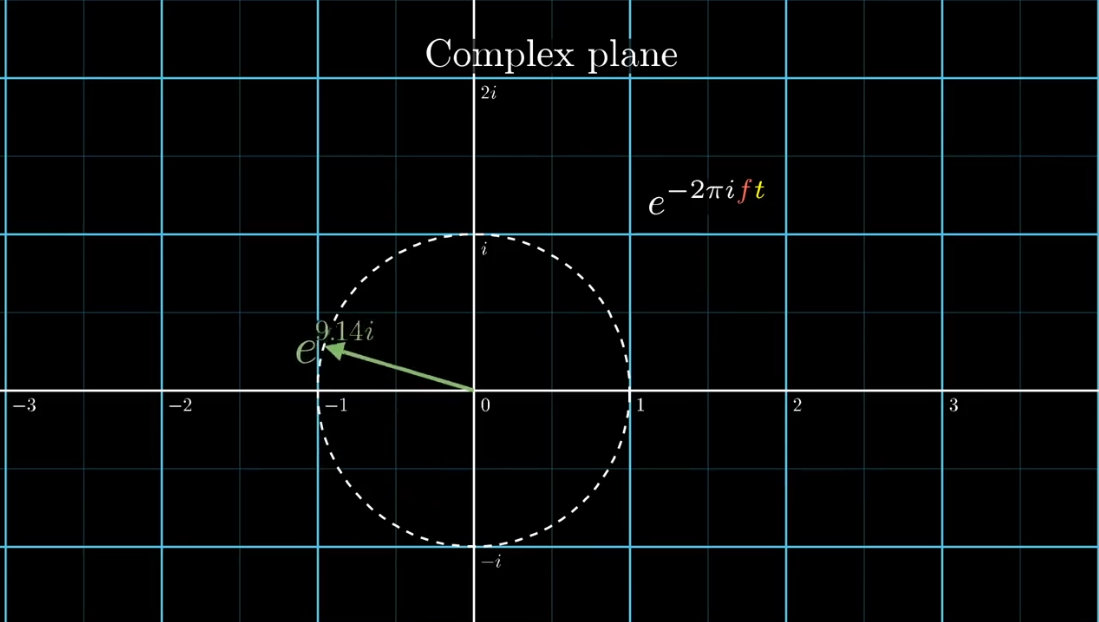
\includegraphics[width=0.8\textwidth]{figures/dft3.png}    
  \caption*{Добавим множитель $f$.}        
\end{figure} 

Пусть теперь модуль нашего вектора не $1$ а некоторая функция $g(t)$ (для неё мы и делаем преобразование
Фурье).

\begin{figure}[H]    
  \centering    
  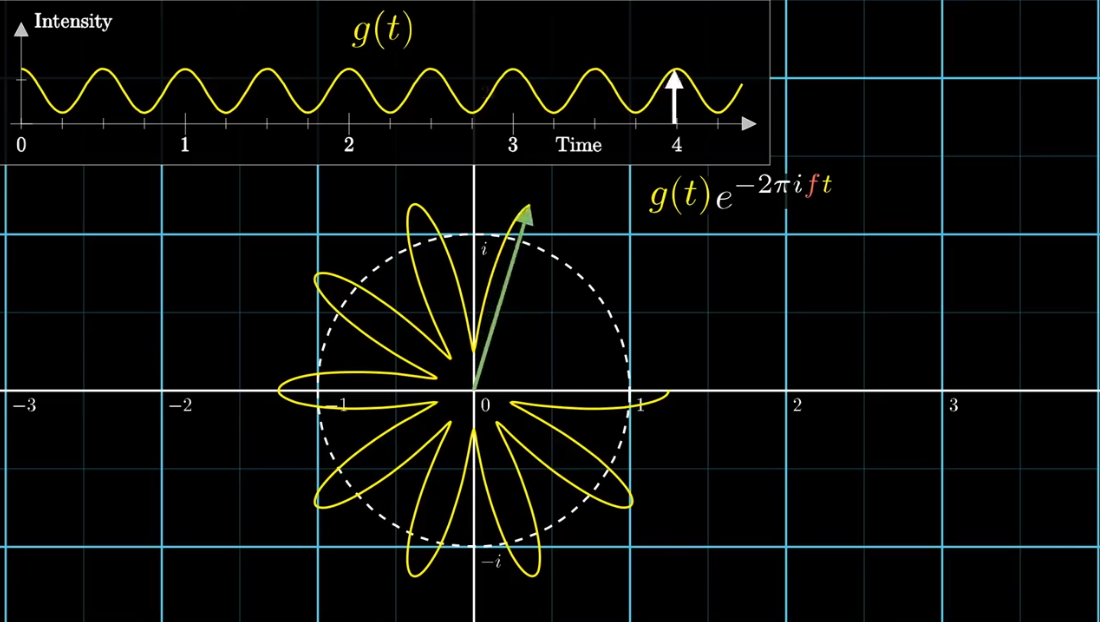
\includegraphics[width=0.8\textwidth]{figures/dft4.png}    
  \caption*{Добавим множитель $g(t)$.}        
\end{figure} 

Как мы видим из рисунка, наша функция принимает различные значения, но нам нужно как-то охарактеризовать 
это множество значений в зависимости от параметра $f$. Для этого мы возьмём некоторый дискретный набор
значений функции и получим среднее значение.

\begin{figure}[H]    
  \centering    
  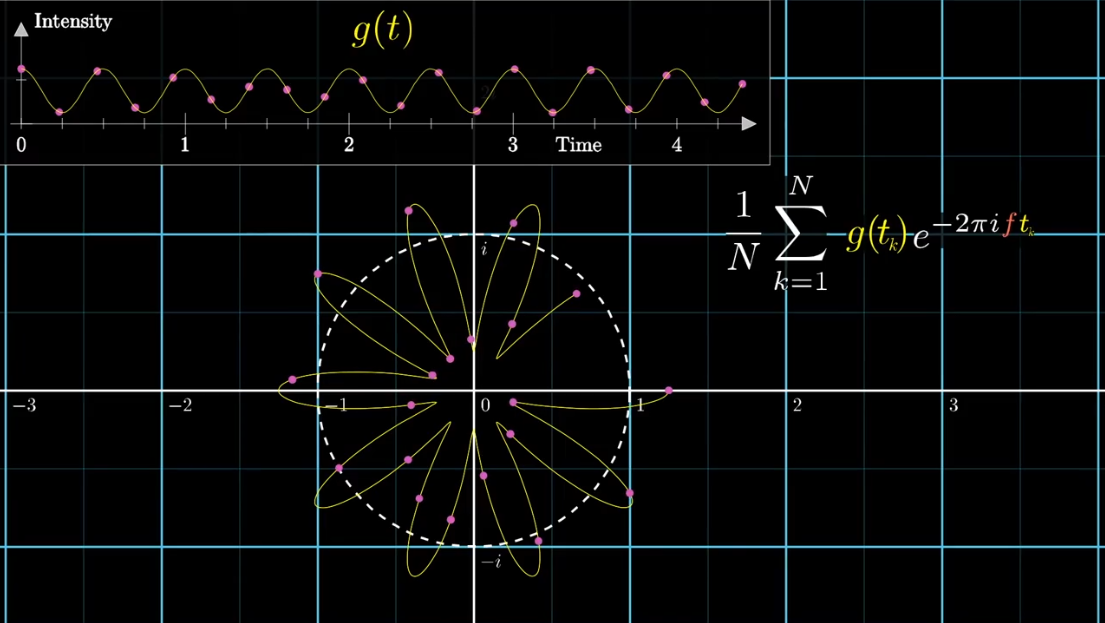
\includegraphics[width=0.8\textwidth]{figures/dft5.png}    
  \caption*{Усредним наши значения.}        
\end{figure} 

Геометрический смысл такой формулы --- центр масс системы точек (розовые точки на предыдущем рисунке).
Получается, наша полученная функция теперь описывает положение центра масс системы в зависимости от
параметра $f$.

При $N \to \infty$ мы получаем интеграл. Осталась одна важная деталь: прямое преобразование Фурье --- 
это наша построенная функция, но без множителя $\frac{1}{N}$.

\begin{figure}[H]    
  \centering    
  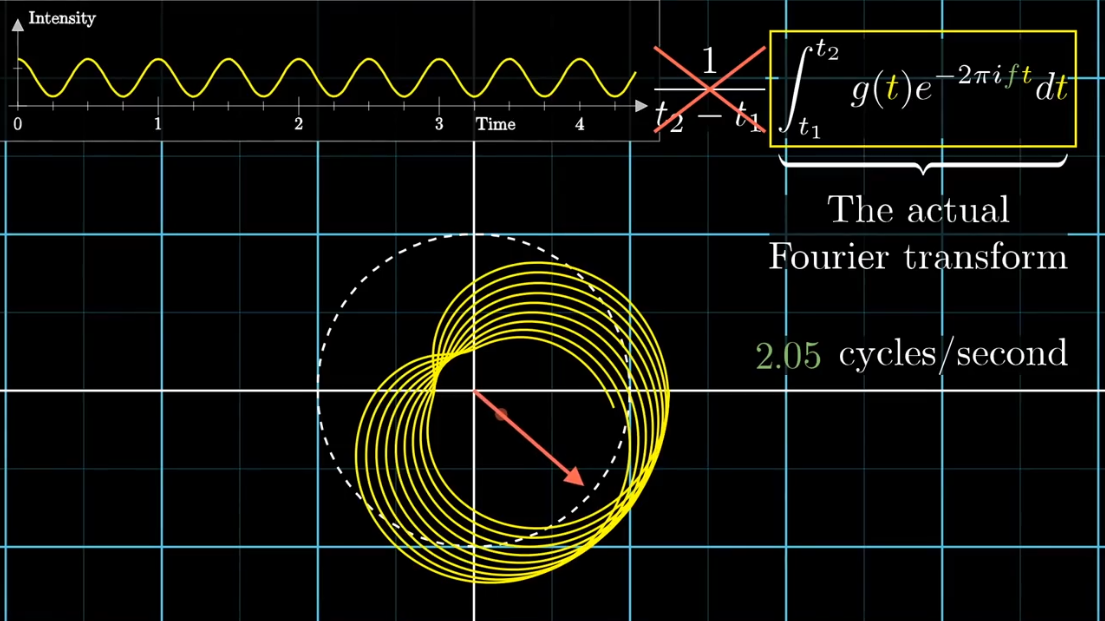
\includegraphics[width=0.8\textwidth]{figures/dft6.png}    
  \caption*{Уберём множитель $\frac{1}{N}$.}        
\end{figure} 

Что теперь мы получили? На самом деле, теперь, чем дольше в нашей функции присутствует функция на
определённой частоте, тем больше у нас будет значение после преобразования Фурье.

\begin{figure}[H]    
  \centering    
  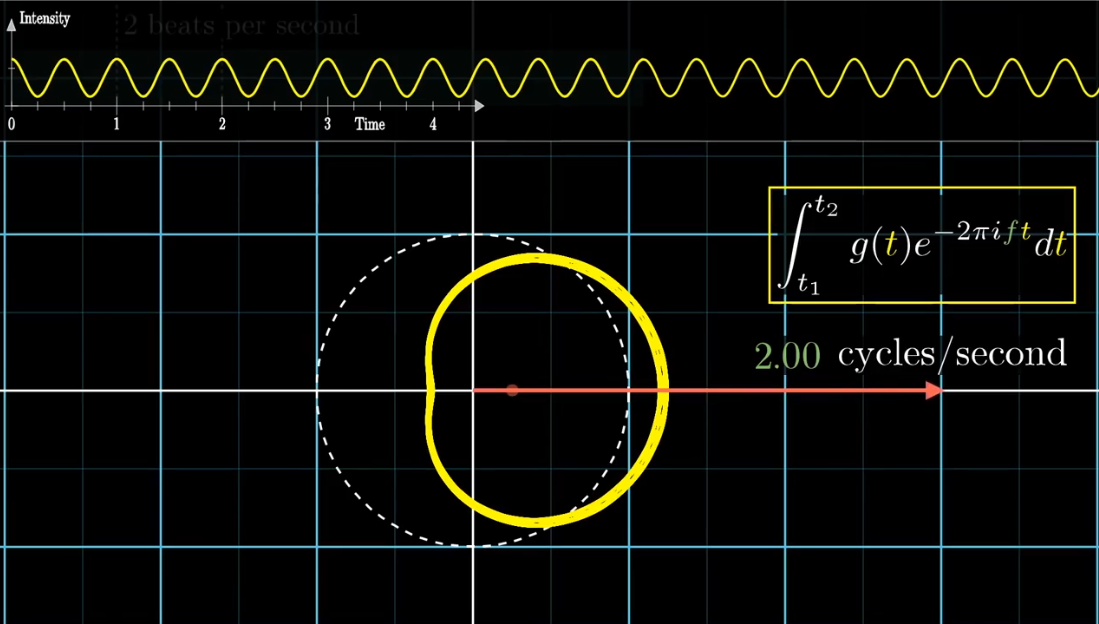
\includegraphics[width=0.8\textwidth]{figures/dft7.png}    
  \caption*{Частота нашей функции совпала с $f$, так что красный вектор (наше значение после Фурье) остаётся
  на месте, но растёт.}        
\end{figure} 

Итого мы по нашей исходной функции зависимости от $t$ построили функцию зависимости от частоты $f$.
В формуле дискретного преобразования Фурье частота $f$ указана неявно в виде $\frac{k}{N}$, а времени
$t$ соответствует $n$.

\begin{figure}[H]    
  \centering    
  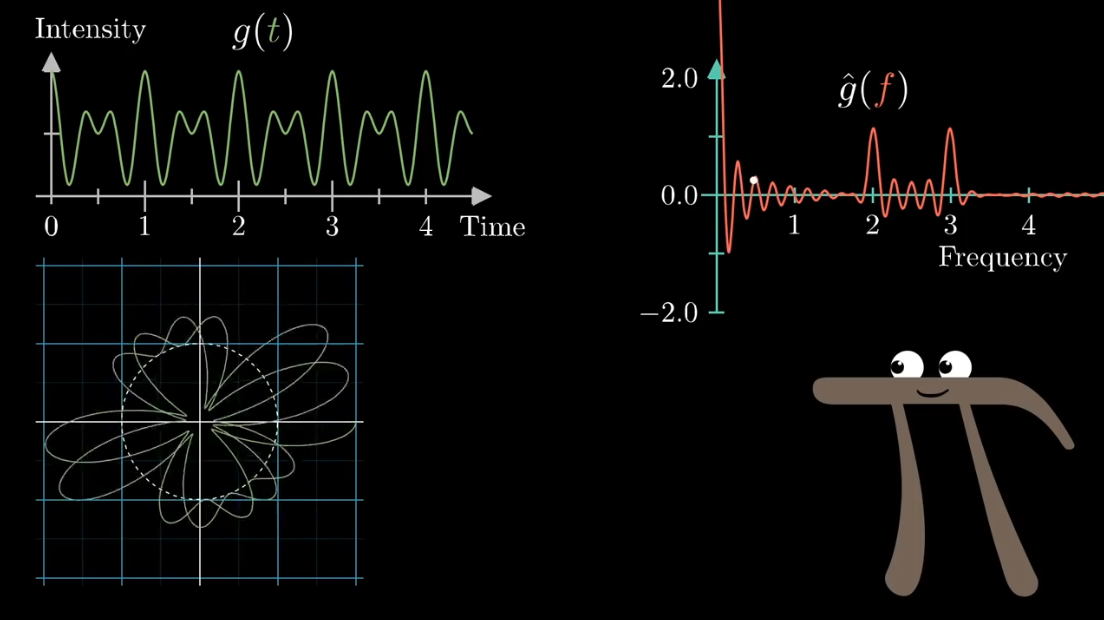
\includegraphics[width=0.8\textwidth]{figures/dft8.png}    
  \caption*{Итого}        
\end{figure} 

Часть с картинками закончилась, дальше формулы.

Аналогично можно ввести обратное преобразование Фурье:
\[
  x_{n} = \frac{1}{N} \sum_{k=0}^{N - 1} X_{k} e^{\frac{2\pi i}{N} kn}
.\] 

В процессе построения преобразования Фурье мы рассматривали некоторое множество значений нашей функции, так
вот это множество, на самом деле, является множеством значений на комплексных корнях из $1$ $n$-ой степени.
Это легко понять, обратившись к части с картинками. Действительно, мы при построении домножили наш
вектор $e^{-2\pi i t}$ на значение нашей функции $g(t)$. Т. е. фактически натянули нашу функцию 
на окружность, который описывает единичный вектор в комплексной плоскости.

\begin{figure}[H]    
  \centering    
  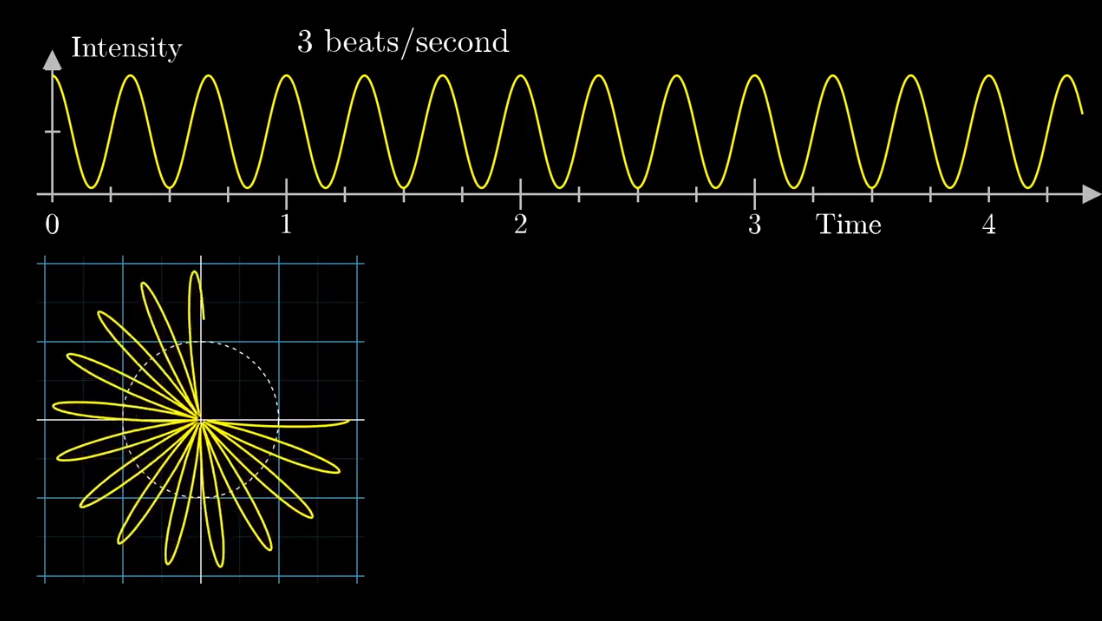
\includegraphics[width=0.8\textwidth]{figures/dft9.png}    
  \caption*{<<Натягиваем>> нашу функцию на окружность, которую описывает единичный вектор в комплексной
  плоскости.}        
\end{figure} 

\begin{remark}
  Сумма всех корней вида $w_{n}^{k} = e^{\frac{2\pi i k}{n}}, k = 0\ldots n - 1$ равна нулю.
\end{remark}
\begin{proof}
  Это напрямую следует из того, как мы выбираем наши точки на комплексной окружности. Фактически, мы
  делим её этими точками на $n$ дуг равной длины. В итоге эти точки образуют равносторонний многоугольник.
  Если просуммируем его вершины как вектора, получим в итоге $0$.
\end{proof}

\subsection{Быстрое преобразование Фурье.}
Пусть у нас есть многочлен степени $n$, где $n$ --- степень двойки.
\[
  A(x) = a_0 x^{0} + a_1 x^{1} + \ldots + a_{n-1} x^{n-1}
.\] 
Разделяем его на два многочлена:
\begin{gather*}
  A_0(x) = a_0 x^{0} + a_2 x^{1} + \ldots + a_{n-2} x^{\frac{n}{2} - 1} \\
  A_1(x) = a_1 x^{0} + a_3 x^{1} + \ldots + a_{n-1} x^{\frac{n}{2} - 1}
\end{gather*}

Для которых выполняется:
\[
  A(x) = A_0(x^2) + x A_1(x^2)
.\] 

Мы уже выяснили ранее, что дискретное преобразование Фурье для многочлена --- его значение на 
комплексных корнях единицы, тогда c учётом $w_{n}^{k} = e^{\frac{2\pi k}{n}} = (w_{n}^{1})^{k}$ получаем:
\[
  DFT(a_0, a_1, \ldots, a_{n-1}) = (A(w_{n}^{0}), A(w_{n}^{1}), \ldots, A(w_{n}^{n-1})) 
.\] 
Докажем вспомогательное утверждение:
\begin{remark}
 \[
  DFT(A \cdot B) = DFT(A) \cdot DFT(B)
 .\]   
\end{remark}
\begin{proof}
  Следует из того, что в каждой точке при умножении многочленов их значения перемножаются, т. е.
  \[
    (A \cdot B)(x) = A(x) \cdot B(x)
  .\] 
\end{proof}

Перейдём к саму алгоритму. Из неравенства для $A(x)$ видно, что если мы научимся за линию считать 
$A(x)$ из посчитанных на предыдущем шаге  $A_0(x^2)$ и $A_1(x^2)$, то асимптотика алгоритма будет
$O(n \log n)$.

Пусть $\{ y_{k}^{0}\}_{k = 0}^{\frac{n}{2} - 1} = DFT(A_0), \{ y_{k}^{1}\}_{k = 0}^{\frac{n}{2} - 1} = DFT(A_1)$.

Найдём выражение для $DFT(A) = \{ y_{k} \}_{k=0}^{n-1}$:
Для первой половины коэффициентов по определению:
\[
  y_{k} = A(w_{n}^{k}) = A_0(w_{n}^{2k}) + w_{n}^{k} \cdot A_1(w_{n}^{2k}) = y_{k}^{0} + w_{n}^{k} y_{k}^1, 
  \text{ при } k = 0\ldots \frac{n}{2} - 1
.\] 

Учитывая $w_{n}^{n} = 1, w_{n}^{\frac{n}{2}} = -1$:
\begin{multline*}
  y_{k + \frac{n}{2}} = A\left(w_{n}^{k + \frac{n}{2}}\right) = A_0(w_{n}^{2k+n}) + w_{n}^{k+\frac{n}{2}} 
  A_1(w_{n}^{2k+n}) \\= A_0(w_{n}^{2k} w_{n}^{n}) + w_{n}^{k} w_{n}^{\frac{n}{2}} A_1(w_{n}^{2k} w_{n}^{n}) =
  A_0(w_{n}^{2k}) - w_{n}^{k} A_1(w_{n}^{2k}) = y_{k}^{0} - w_{n}^{k} y_{k}^{1}
\end{multline*}
Полученные преобразования называют <<преобразованием бабочки>>.

Таким образом, задача DFT сводится к двум подзадачам и пересчёту индексов по формулам выше.
Обратное DFT ничем не отличается от прямого, кроме формулы пересчёта коэффициентов.
Её можно найти, посчитав обратную матрицу к матрице перехода при прямом DFT.

Некоторые оптимизации:
\begin{enumerate}
  \item Для начала заметим, что на первом уровне рекурсии к первому массиву относятся элементы на чётных
    позициях, т. е. те, у которых младшие биты позиции равны нулю, а ко второму массиву --- те, у которых
    младшие биты позиции равны единице. На следующем шаге аналогично со второй позицией и т. д. Таким образом,
    мы можем переупорядочить наш набор элементов так, чтобы элементы занимали свои позиции после окончания
    рекурсии. Например, для $n = 8$ вид следующий:
    \[
      a = \left\{ \left[ \left( a_0, a_4 \right), \left( a_2, a_6 \right)   \right], \left[ \left( a_1, a_5 \right), \left( a_3, a_7 \right)   \right]   \right\} 
    .\] 
    Пусть теперь после выполнения алгоритма к каждой половине у нас такой вид массива на последнем шаге:
    \[
    a = \left\{ \left[ y_0^0, y_1^0, y_2^0, y_3^0,\right], \left[ y_0^1, y_1^1, y_2^1, y_3^1,\right]  \right\} 
    .\] 
    Теперь нам осталось объединить оба массива. Элементы стоят так, что мы можем сделать это прямо на 
    месте без доп. памяти с помощью преобразования, полученного ранее:
    \[
      a = \left\{ \left[ y_0^0 + w_{n}^{0}y_0^1, y_1^0, y_2^0, y_3^0,\right], \left[ y_0^0 - w_{n}^0 y_0^{1}, y_1^1, y_2^1, y_3^1,\right]  \right\} 
    .\] 
    Аналогичным образом для других элементов массива. Таким образом, мы избавились от рекурсии вовсе: 
    сделали поразрядную обратную сортировку, а потом применили преобразование бабочки для всех уровней
    рекурсии.
  \item Можно предпосчитать обратную сортировку для битов, если функция вызывается часто. 
  \item Предпосчитать все нужные степени $w_{n}^{k}$.
\end{enumerate}

\subsection{Умножение многочленов.}
\begin{remark}
  Для произведения двух многочленов справедлива формула:
  \[
    A \cdot B = DFT^{-1} \left( DFT(A) \cdot DFT(B)  \right) 
  .\] 
\end{remark}
\begin{proof}
  Следует из утверждения, что $DFT(A \cdot B) = DFT(A) \cdot DFT(B)$.
  Здесь и в формуле произведения подразумевается почленное умножение для DFT.
\end{proof}

\begin{remark}
  Асимптотика такого умножения --- $O(n \log n)$.
\end{remark}
\begin{proof}
  Каждое DFT выполняется за $O(n \log n)$, почленное умножение многочленов за $O(n)$. 
\end{proof}

